\documentclass[a4paper,11pt]{article}
\usepackage[T1]{fontenc}
\usepackage[utf8]{inputenc}
\usepackage{lmodern}
% \usepackage{hyperref} % fucking warnings
\usepackage{graphicx}
\usepackage{graphics}
\usepackage{rotating}
\usepackage{listings}
\usepackage{color}
\usepackage{listings}
\usepackage{amsthm}
\usepackage{amsmath}
\usepackage{amssymb}
\usepackage{algorithmic}
\usepackage{datatool}
\usepackage{caption}
\usepackage{subcaption}

% \newcommand{\encode}[1] {{ {}_{\llcorner}{#1}_{\lrcorner}}}

\title{Numerical Linear Algebra (CSE-6643) - Midterm take home exam}
\author{Arash Rouhani (rarash@gatech.edu) - gtid: 902951864}


\begin{document}

\maketitle

\section{Part I}

blah blah

\section{Part II}

\subsection{a}

Here is an algorithm to generate a matrix $A$ with the given singular values
$\Sigma$. Generate two random unitary matrixes $U$ and $V$ and let $A = U
\Sigma V^*$. The way you generate the unitary matrices could be like this:

Let $P=I$ be a projector which is gonna make sure of the orthogonality of the
vectors we generate. For each $i=1 \to n$, we first randomly create size $n$
row vector $a_i$. Now to ensure that it's orthogonal to all previous vectors,
we multiply it by $P$. To ensure that future vectors will be orthogonal to the
current vector we set $P$ to $P P_{\perp a_i}$. Also, after we have projected
$a_i$ we also normalize it. Hence each vector we create is orthogonal to all
previous ones and it's also of length 1 because it's normalized. Constructing
a matrix consisting of these $n$ vectors will be unitary.

In practice this algorithm is superflous, because this is exactly
how the stable gram schmidt generates $Q$, only that the $a_i$ vectors isn't
random but based on the input, so we create our unitary matrixes by feeding
random data to stable gram schmidt and only looking at it's $Q$ output.

\subsection{b}

I found it interesting to look at these values in the two algorithms $QR$
factorization.

\begin{itemize}
  \item Look at the norms of the produced $Q$s. Ideally they should be $1$.
  \item Define two matrices $\Delta Q$ and $\Delta R$ to $Q_{classic} -
    Q_{stable}$ and $R_{classic} - R_{stable}$ respectivly. Then plot both
    their row and column medians.

\end{itemize}

Let's first look at the data for $n=100$ and then see if
the pattern is partiuclarly different for $n=150$.

\subsubsection{$n=100$}
\begin{table}[h]
  \begin{tabular}{r|c|c|c|}
    \multicolumn{1}{r}{}
     & \multicolumn{1}{c}{$Q_{classic}$ }
     & \multicolumn{1}{c}{$Q_{stable}$}
     & \multicolumn{1}{c}{$Q_{householder}$} \\
    \cline{2-4}
    $n=100$ & \input{data/norm-q-classi-100.dat}
            & \input{data/norm-q-stable-100.dat}
            & \input{data/norm-q-househ-100.dat}
            \\ \cline{2-4}
    $n=150$ & \input{data/norm-q-classi-150.dat}
            & \input{data/norm-q-stable-150.dat}
            & \input{data/norm-q-househ-150.dat}
            \\ \cline{2-4}
  \end{tabular}
  \caption{Norms for the different unitary $Q$ matrices}
  \label{tab:norms}
\end{table}

\begin{table}[h]
  \begin{tabular}{r|c|c|c|}
    \multicolumn{1}{r}{}
     & \multicolumn{1}{c}{$Q_{classic}$ }
     & \multicolumn{1}{c}{$Q_{stable}$}
     & \multicolumn{1}{c}{$Q_{householder}$} \\
    \cline{2-4}
    $n=100$ & \input{data/std-q-classi-100.dat}
            & \input{data/std-q-stable-100.dat}
            & \input{data/std-q-househ-100.dat}
            \\ \cline{2-4}
    $n=150$ & \input{data/std-q-classi-150.dat}
            & \input{data/std-q-stable-150.dat}
            & \input{data/std-q-househ-150.dat}
            \\ \cline{2-4}
  \end{tabular}
  \caption{The standard deviation for the values of $A-QR$}
  \label{tab:stds}
\end{table}

\newcommand{\genfig}[3] {{
    \begin{figure}
            \centering
            \begin{subfigure}[b]{1.0\textwidth}
                    \includegraphics[width=\textwidth]{fig/#1-#2-100}
                    \caption{$n = 100$}
            \end{subfigure}
            \begin{subfigure}[b]{1.0\textwidth}
                    \includegraphics[width=\textwidth]{fig/#1-#2-150}
                    \caption{$n = 150$}
            \end{subfigure}
            \caption{Medians of the columns of $\Delta #2$ #3}\label{fig:#1}
    \end{figure}
  }}

\genfig{log-median-col}{Q}{logarithmized}
\genfig{median-row}{Q}{}
\genfig{log-median-col}{R}{logarithmized}
\genfig{log-median-row}{R}{logarithmized}

% \begin{figure}
%         \centering
%         \begin{subfigure}[b]{1.0\textwidth}
%                 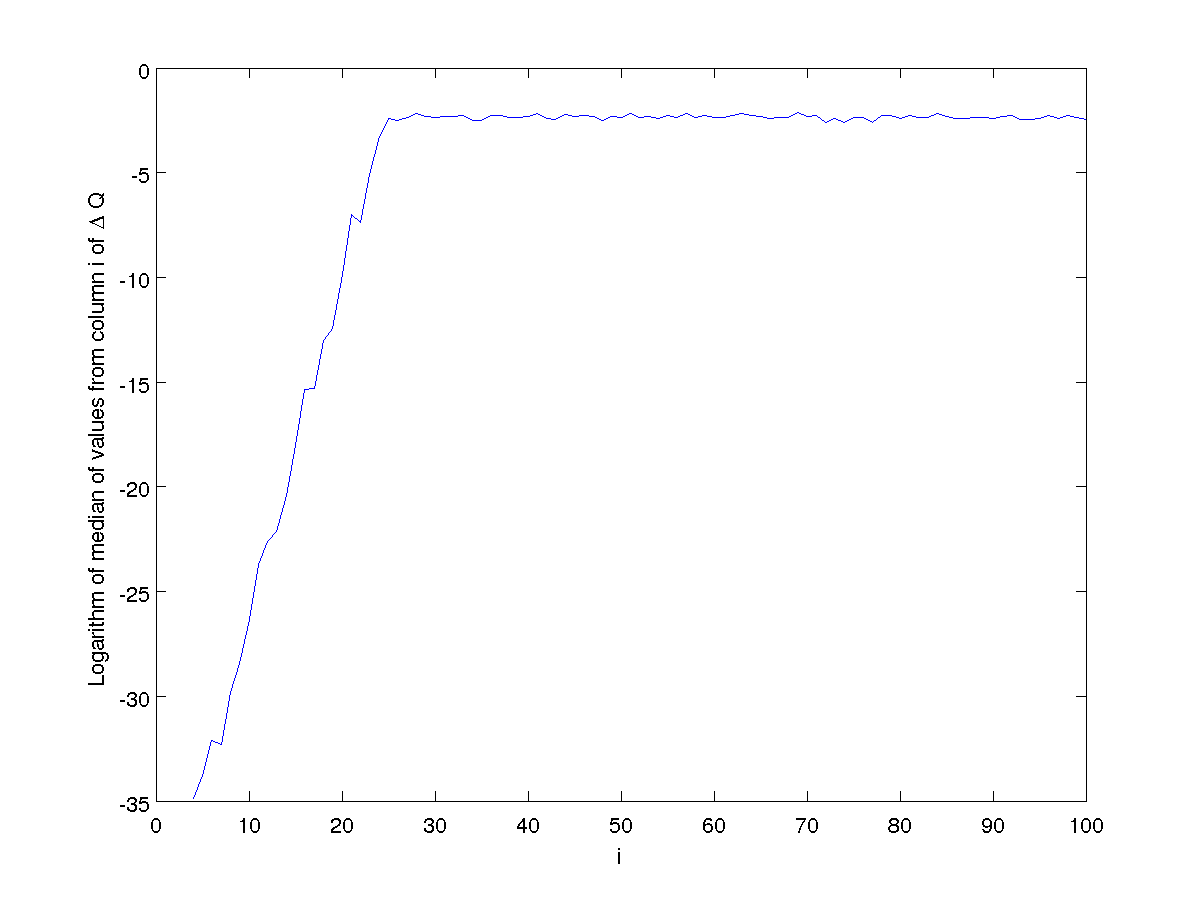
\includegraphics[width=\textwidth]{fig/log-median-col-Q-100}
%                 \caption{$n = 100$}
%         \end{subfigure}
%         \begin{subfigure}[b]{1.0\textwidth}
%                 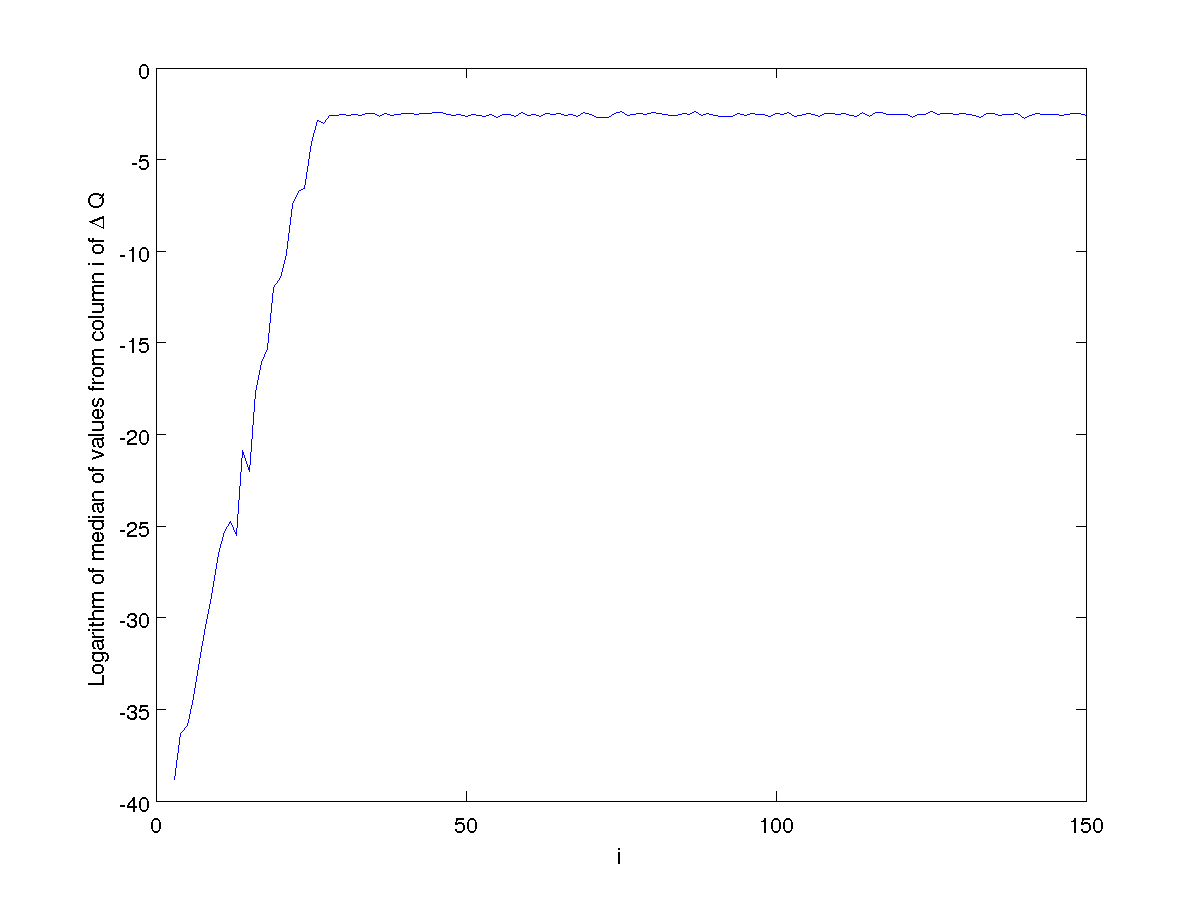
\includegraphics[width=\textwidth]{fig/log-median-col-Q-150}
%                 \caption{$n = 150$}
%         \end{subfigure}
%         \caption{Medians of the columns of $\Delta Q$ logarithmized}\label{fig:med-q-col}
% \end{figure}

% The 2-norm for is and
% \input{data/norm-q-stable.dat} for .

% The plots 

\subsubsection{$n=150$}

% Now, loop through  $a_i$ $P:= $

% \begin{algorithm}
%   \FOR{$i = 1 \to 10$}
%     blah
%   \ENDFOR
%   \caption{How go generate unitary matrix}
% \end{algorithm}

\end{document}
